% !TeX root = ../../../book.tex
\subsection{平面上的线}

拿一张干净的纸、一支笔和一把尺子。这张纸上有多少个区域?只有一个,对吧?在纸上画一条直线。现在有两个区域。再画一条与第一条直线相交的直线。现在有多少个区域?数一数,总共有四个。绘制第三条直线线,与前两条直线相交,但不过前两条直线的交点。(也就是说,总共应该有三个交点。)现在有多少个区域?你能在不数的情况下预测答案吗?当有 $4$ 条直线时会怎样?$5$ 个呢?$100$ 个呢?我们如何解这道题并最终解决它?让我们给出一个更正式的陈述,以确保我们用同样的方式思考:

考虑无限平面(二维表面)上的 $n$ 条直线,互不\emph{平行}且没有两条以上的线过\emph{同一交点}。这些直线分割出多少个不同区域?

当 $n$ 很小时(例如,$n$ 不超过 $5$),我们可以手工画一些例子,让这些例子来引导我们的直觉,对\emph{任意} $n$ 值进行一般论证。(请注意,此策略与我们在上一题中所做的非常相似:识别较小案例的模式,识别这些案例中可以泛化的相关部分,然后抽象为任意案例。)具体来说,我们想尝试确定一幅图中的区域数量如何\emph{取决于}线条较少的图中的区域数量。当我们画一条新的直线时会发生什么?我们能否确定它是如何改变现有区域的?我们能以某种方式计算一下它创建了多少个区域吗?在继续阅读之前,请自行对本题进行一些调研。如果你得出一些结果,请将你的工作与我们下面遵循的步骤进行比较。 

让我们从 $n = 2$ 开始。我们知道一条直线将平面分为 $2$ 个区域;当我们添加第二条直线时会发生什么?我们知道会有 $4$ 个区域,因为我们可以画出图形并数出这些区域:

\begin{center}
    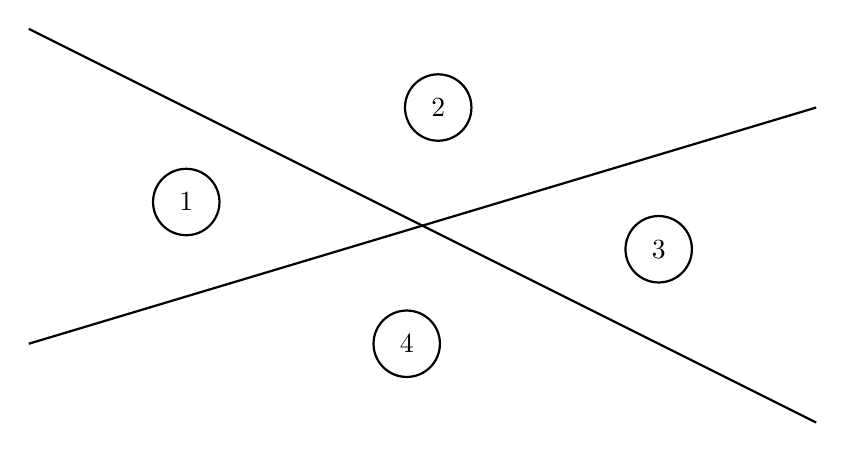
\begin{tikzpicture}[thick]
        \draw (-5,2.5) -- (5,-2.5);
        \draw (-5,-1.5) -- (5,1.5);
        \node[draw,circle,minimum size=24pt,inner sep=0,anchor=center] at (-0.2,-1.5) {$4$};
        \node[draw,circle,minimum size=24pt,inner sep=0,anchor=center] at (3,-0.3) {$3$};
        \node[draw,circle,minimum size=24pt,inner sep=0,anchor=center] at (-3,0.3) {$1$};
        \node[draw,circle,minimum size=24pt,inner sep=0,anchor=center] at (0.2,1.5) {$2$};
    \end{tikzpicture}
\end{center}

然而,这只是两条直线相交的一种\emph{具体情况}。我们怎么知道无论我们如何画这两条线,\emph{总能}得到四个区域?也就是说,我们能否以某种方式结合直线数量 $n = 2$ 这一事实来描述这是\text{如何}发生的?思考一下!

下面是我们的方法。请注意,当我们添加第二条直线时,每个已经存在的区域都会被分成两部分,并且\emph{无论你如何绘制直线},只要我们确保两条直线不平行,结果都是这样。也就是说,如果我们用一条直线将平面分成两个区域,

\begin{center}
    \begin{tikzpicture}[thick]
        \draw (-5,2.5) -- (5,-2.5);
        \node[draw,circle,minimum size=24pt,inner sep=0,anchor=center] at (-3,0.3) {$1$};
        \node[draw,circle,minimum size=24pt,inner sep=0,anchor=center] at (0.2,1.5) {$2$};
    \end{tikzpicture}
\end{center}

然后添加一条新的直线会将每个现有区域分成两部分。这会向整个平面添加两个新的区域,总共四个区域:

\begin{center}
    \begin{tikzpicture}[thick]
        \draw (-5,2.5) -- (5,-2.5);
        \draw [color=red] (-5,-1.5) -- (0,0)  node[midway,below,sloped]{分割区域 1}
        -- (5,1.5) node[midway,above,sloped]{分割区域 2} ;
        \node[draw,circle,minimum size=24pt,inner sep=0,anchor=center,color=red] at (-0.2,-1.5) {$4$};
        \node[draw,circle,minimum size=24pt,inner sep=0,anchor=center,color=red] at (3,-0.3) {$3$};
        \node[draw,circle,minimum size=24pt,inner sep=0,anchor=center] at (-3,0.3) {$1$};
        \node[draw,circle,minimum size=24pt,inner sep=0,anchor=center] at (0.2,1.5) {$2$};
    \end{tikzpicture}
\end{center}

当 $n = 3$ 时呢?在这种情况下,我们需要考虑向具有两条直线和四个区域的图形中添加第三条直线。我们想要提出一个不依赖于线的特定排列的论证,因此我们最终唯一能用的事实是线之间互不平行,且任何交点仅位于两条线(而不是三条或更多)上。不过,就目前而言,查看特定的线条排列会有所帮助,以便我们讨论相同的图形;我们可以利用对这个特定图形的观察来指导我们的一般论证。让我们从下方具有两条直线的图开始,向其中添加第三条线,我们让第三条线的交点都在初始交点``附近''或在图的范围内,这样我们就缩放图形了:

\begin{center}
    \begin{tikzpicture}[thick]
        \draw (-5,2.5) -- (5,-2.5);
        \draw (-5,-1.5) -- (5,1.5);
        \draw [color=red] (-5,1) -- (-1.8085,0.9043) node[midway,below,sloped]{\small 分割区域 1} 
        -- (2.5758,0.7727) node[midway,above,sloped]{\small 分割区域 2}
        -- (5,0.7) node[midway,below,sloped]{\small 分割区域 3};
        \node[draw,circle,minimum size=16pt,inner sep=0,anchor=center] at (-0.2,-1.5) {$4$};
        \node[draw,circle,minimum size=16pt,inner sep=0,anchor=center] at (3,-0.3) {$3$};
        \node[draw,circle,minimum size=16pt,inner sep=0,anchor=center] at (-3,-0.3) {$1$};
        \node[draw,circle,minimum size=16pt,inner sep=0,anchor=center] at (0.2,2) {$2$};
        \node[draw,circle,minimum size=16pt,inner sep=0,anchor=center,color=red] at (-4,1.45) {$5$};
        \node[draw,circle,minimum size=16pt,inner sep=0,anchor=center,color=red] at (0.1,0.45) {$6$};
        \node[draw,circle,minimum size=16pt,inner sep=0,anchor=center,color=red] at (4.61,1.05) {$7$};
    \end{tikzpicture}
\end{center}

很明显现在我们有 $7$ 个区域。我们将第三条线设置为不同的颜色,以便我们可以识别``新''区域出现的位置:一个区域(下方区域,区域 $4$)保持不变,但其他三个区域被一分为二,每个``分割''都会让我们的计数加 $1$(原来有 $1$ 个区域,现在有 $2$ 个)。如果我们以不同的方式绘制这条直线会怎样?

\begin{center}
    \begin{tikzpicture}[thick]
        \draw (-5,2.5) -- (5,-2.5);
        \draw (-5,-1.5) -- (5,1.5);
        \draw [color=red] (0,2.5) -- (-0.8333,0.4167) node[midway,right,sloped,rotate=-90]{\small 分割区域 2} 
        -- (-1.1364,-0.341) node[midway,left,sloped,rotate=-90]{\small 分割区域 1}
        -- (-2,-2.5) node[midway,right,sloped,rotate=-90]{\small 分割区域 4}; 
        \node[draw,circle,minimum size=16pt,inner sep=0,anchor=center] at (-0.2,-1) {$4$};
        \node[draw,circle,minimum size=16pt,inner sep=0,anchor=center] at (3,-0.3) {$3$};
        \node[draw,circle,minimum size=16pt,inner sep=0,anchor=center] at (-3,-0.3) {$1$};
        \node[draw,circle,minimum size=16pt,inner sep=0,anchor=center] at (1,2) {$2$};
        \node[draw,circle,minimum size=12pt,inner sep=0,anchor=center,color=red] at (-0.7,0.05) {$5$};
        \node[draw,circle,minimum size=16pt,inner sep=0,anchor=center,color=red] at (-1.5,1.8) {$6$};
        \node[draw,circle,minimum size=16pt,inner sep=0,anchor=center,color=red] at (-2.5,-1.4) {$7$};
    \end{tikzpicture}
\end{center}

同样的现象再次发生,其中一个区域保持不变,但其他三个区域一分为二。(我们怎么知道没有任何其他区域未绘制在我们这个比例的图形内?这并不像看上去的那么容易回答,值得深刻考虑。)尝试三条线的其他排列方式,并试图说服自己这种情况总会发生;此外,思考一下\emph{为什么}会出现这种情况,以及我们\emph{如何}解释这种情况一定会发生。不过,在给出一般性解释之前,我们先来看另一个小案例。

当 $n = 4$ 时,我们从 $3$ 条直线和 $7$ 个区域的平面开始,然后添加第四条直线,该线不与任何现有线平行,并且不穿过任何现有交点。同样,我们想要提出一个与特定的线条排列无关的论证,但是查看下面的具体图形将有助于引导我们的直觉来提出该论证:

\begin{center}
    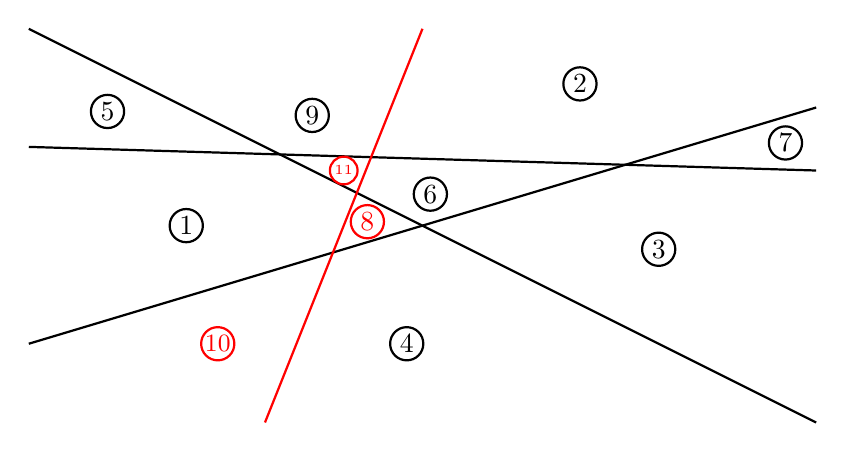
\begin{tikzpicture}[thick]
        \draw (-5,2.5) -- (5,-2.5);
        \draw (-5,-1.5) -- (5,1.5);
        \draw  (-5,1) -- (5,0.7);
        \draw [color=red] (0,2.5) -- (-2,-2.5);
        \node[draw,circle,minimum size=12pt,inner sep=0,anchor=center] at (-0.2,-1.5) {$4$};
        \node[draw,circle,minimum size=12pt,inner sep=0,anchor=center] at (3,-0.3) {$3$};
        \node[draw,circle,minimum size=12pt,inner sep=0,anchor=center] at (-3,0) {$1$};
        \node[draw,circle,minimum size=12pt,inner sep=0,anchor=center] at (2,1.8) {$2$};
        \node[draw,circle,minimum size=12pt,inner sep=0,anchor=center] at (-4,1.45) {$5$};
        \node[draw,circle,minimum size=12pt,inner sep=0,anchor=center] at (-1.4,1.4) {$9$};
        \node[draw,circle,minimum size=10pt,inner sep=0,anchor=center,color=red] at (-1,0.7) {\tiny $11$};
        \node[draw,circle,minimum size=12pt,inner sep=0,anchor=center] at (4.61,1.05) {$7$};
        \node[draw,circle,minimum size=12pt,inner sep=0,anchor=center,color=red] at (-0.7,0.05) {$8$};
        \node[draw,circle,minimum size=12pt,inner sep=0,anchor=center] at (0.1,0.4) {$6$};
        \node[draw,circle,minimum size=12pt,inner sep=0,anchor=center,color=red] at (-2.6,-1.5) {\small $10$};
    \end{tikzpicture}
\end{center}

请注意,三个原始区域保持不变(区域 $3$、区域 $5$ 和区域 $7$),其他四个区域一分为二。你注意到这里存在一个模式吗?似乎对于我们检查过的每个 $n$,添加第 $n$ 条线会使 $n-1$ 个区域保持不变,而其余区域则被一分为二。让我们尝试解释为什么会出现这种情况。请记住,当我们绘制 $n$ 条直线时,我们试图确定出现了多少个区域,因此让我们为该值分配一个``名称'',以便我们可以引用它;假设 $R(n)$ 表示在平面上绘制 $n$ 条直线所创建的区域数,且没有两条线平行,并且没有交点在两条以上的线上。在上面示例中,我们考虑了 $n$ 的较小取值,并研究了添加新的直线时会发生什么变化;也就是说,我们可以通过已知 $R(n - 1)$ 算出 $R(n)$ 的值。让我们整理一下我们的观察结果,以便它们适用于\emph{任意} $n$ 值。

假设我们已知 $R(n)$。(为什么我们可以这样做?对于某个特定的 $n$,我们是否确实知道 $R(n)$ 的特定值?这个值是什么?如何知道的?)假设我们在平面上有一个\emph{任意} $n$ 线图,满足上面题目陈述中给出的两个条件。这些直线创建了多少个区域?是的,正是 $R(n)$。现在,当我们添加第 $(n + 1)$ 条直线时会发生什么?关于这条线以及它如何改变图形,我们可以确定什么?其实,我们真正掌握的唯一信息是:

\begin{enumerate}[label=(\alph*)]
    \item 这条新的直线与现有的 $n$ 条直线中的任何一条都不平行;
    \item 这条新的直线不经过任何现有的交点。
\end{enumerate}

现在,条件 (a) 告诉我们这条新的直线必须与\emph{所有}现有的 $n$ 条直线线相交;平行线不相交,非平行线必然相交于某处。因此,我们必须在图上创建 $n$ 个新的交点。这些交点会与任何现有交点重合吗?不会!这正是条件 (b) 告诉我们的。这两条信息合在一起告诉我们,无论我们如何绘制这条新的直线,只要它满足题目的要求,这条直线上\emph{一定}会出现 $n$ 个``特殊''点。这些特殊点正是新线与现有线的交点。

我们现在想利用这些特殊点来识别图中的新区域。回顾一下我们上面研究的案例:识别新的交点,看看是否可以将它们与新的区域关联起来。也许用圆点标记这些交点并用 $\textbf{×}$ 标记新区域会有所帮助,让它们更容易辨认。我们在下面为你展示了一个示例,其中 $n = 4$。你注意到了什么?你能用这些点来帮助识别添加第 $n$ 条直线后创建了多少新区域吗?思考一下,然后继续阅读。

\begin{center}
    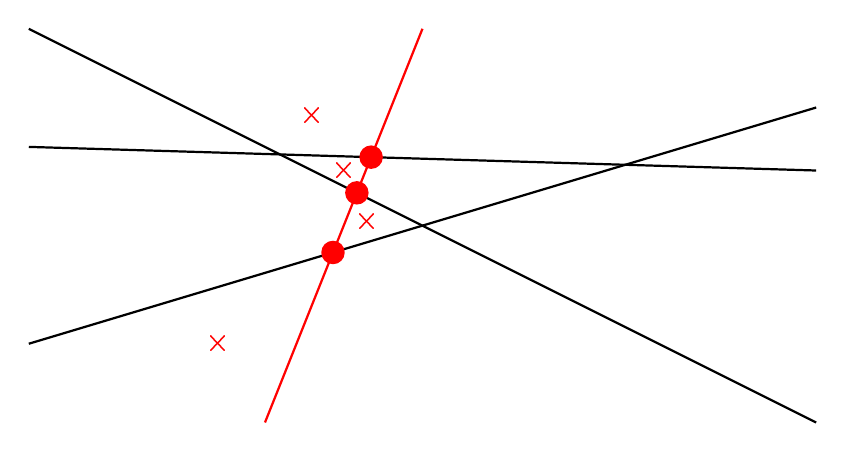
\begin{tikzpicture}[thick]
        \draw (-5,2.5) -- (5,-2.5);
        \draw (-5,-1.5) -- (5,1.5);
        \draw  (-5,1) -- (5,0.7);
        \draw [color=red] (0,2.5) -- (-2,-2.5);
        \node[minimum size=14pt,anchor=center,color=red,very thick] at (-1.4,1.4) {$\textbf{×}$};
        \node[minimum size=14pt,anchor=center,color=red,very thick] at (-1,0.7) {$\textbf{×}$};
        \node[minimum size=14pt,anchor=center,color=red,very thick] at (-0.7,0.05) {$\textbf{×}$};
        \node[minimum size=14pt,anchor=center,color=red,very thick] at (-2.6,-1.5) {$\textbf{×}$};
        \node[fill,circle,inner sep=3pt,color=red] at (-0.6522,0.8696) {};
        \node[fill,circle,inner sep=3pt,color=red] at (-0.8333,0.4167) {};
        \node[fill,circle,inner sep=3pt,color=red] at (-1.1364,-0.341) {};
    \end{tikzpicture}
\end{center}

没错!任意两个相邻新交点之间,都有一条\emph{线段}将一个区域一分为二!剩下的就是确定我们创建了多少个新的此类线段。由于每条线段都将唯一\emph{一个}现有区域一分为二,因此这将准确地告诉我们创建了多少个新区域。我们已知,第 $(n + 1)$ 条直线线创建了 $n$ 个新的交点。想想这些点是如何排列在直线上的。任意两个``连续''点都会创建一条线段,但极点也会创建无限线段(永远延申下去经过这些极点)。总共有多少个?正好是 $n + 1$。(参考上图,$n = 3$。我们看到有 $3$ 个新交点和 $4$ 条新线段,其中两个是无限射线。)这意味着有 $n + 1$ 条线段将区域一分为二,因此我们恰好创建了 $n + 1$ 个新区域!这让我们可以说
\[R(n + 1) = R(n) + n + 1\]
哇,多好的观察啊!我们花了一些时间研究示例并进行了一些几何论证,但最终我们做到了。我们已经确定了这个问题的一些归纳结构;我们发现一个情况如何依赖另一个情况。也就是说,我们发现了 $R(n+1)$ 如何依赖 $R(n)$。这还没有完全解决这个问题,但我们现在已经非常接近了。剩下的就是用类似的表达式替换 $R(n)$,并不断执行此操作,直到达到我们已知的 $R(1) = 2$。观察:

\begin{center}
    \begin{tabular}{rcccccccccc}
        $R(n+1)$ & $=$ &          & &            &     &            &     & $\cancel{R(n-1)}$ & $+$ & $n+1$\\
                 & $=$ &          & &                   &     & $\cancel{R(n-1)}$ & $+$ & $n$ & $+$ & $n+1$\\
                 & $=$ &          & & $\cancel{R(n-2)}$ & $+$ & $(n-1)$           & $+$ & $n$ & $+$ & $n+1$\\
                 & $\vdots$ &     & &  &  &  &  &  &  & \\
                 & $=$ &          & & $\cancel{R(2)}+3$ & $+$ & $\dots$ & $+$ & $n$ & $+$ & $n+1$ \\
                 & $=$ & $R(1)+2$ & $+$ & $3$               & $+$ & $\dots$ & $+$ & $n$ & $+$ & $n+1$ \\
    \end{tabular}
\end{center}

因为我们知道 $R(1) = 2$,所以我们可以说
\[R(n + 1) = 2 + \big(2 + 3 + \dots + n + (n + 1)\big) = 2 + \Bigg(\sum_{k=1}^{n+1}k\Bigg)-1 = 1+\sum_{k=1}^{n+1}k\]
而这正是我们之前研究过的求和公式!(另请注意,我们必须减去 $1$,因为括号中缺少求和的第一项。)回想一下 $\sum_{k=1}^{n} k = \frac{n(n+1)}{2}$,为了表示上面等式中的求和,我们只需将 $n$ 替换为 $n + 1$ 即可。因此,
\[R(n + 1) = 1+\frac{(n+1)(n+2)}{2}\]
我们要进行的最后一步简化是将整个方程中的 $n+1$ 替换为 $n$,因为使用 $R(n)$ 的表达式更有意义(对 $n$ 的值有什么要求?)
\[R(n + 1) = 1+\frac{n(n+1)}{2}\]
最终,我们找到了开头问题的答案!在这个过程中,我们采用了\emph{归纳}技术:我们解释了一个``事实''(即 $R(n + 1)$ 的值)如何\emph{取决于}``前一个事实''(即 $R(n)$ 的值),并使用这些迭代依赖关系进行反向运算,直到达到一个特定的\emph{已知}值,即 $R(1)$。

我们想再次指出,我们在本节中所做的推导和观察只是引导我们的直觉从而得出答案,并不是\emph{严格证明}。问题出在 ``$\dots$'' 身上,省略号不是具体的、``官方''的数学方法来捕获归纳技术背后的归纳过程。此外,我们解决``平面中的线''问题的方法是从 $n - 1$ 条线的图形\emph{开始,构建}一个包含 $n$ 条线的新图;这样可以吗?为什么这实际上告诉了我们有关 $n$ 条线的\emph{任意}图的信息?所有这些图都来自于少了一条线的较小图吗?

在接下来的两章中,我们将学习必要的工具来充分描述我们迄今为止所做事情的严格方法,在那之后的章节中,我们将使用这些工具让数学归纳法变得正式而严谨。不过,现在我们想给出归纳法的启发式定义,并继续研究依赖归纳技术的有趣问题和观察结果。练习这些类型的问题 --- 学习何时识别归纳过程、如何使用它、如何使用该结构来解决问题等等 --- 将在未来非常有帮助,我们不需要深入到数学技术细节。(至少,现在还不需要!)
